\section{Method}

We provide an overview of our method in \cref{fig:method}. Our inputs are a video (also referred to as the "driving video") and a static image.
We apply an off-the-shelf image and video segmentation model\cite{ravi2024sam2} to obtain binary segmentation masks of the foreground object.
For the video, we obtain a segmentation mask for each frame, tracking the relative motion of the masked object.
We use a bounding box approach to calculate the change in position and scale for each frame in the video mask.
Given this per-frame deformation, we can sequentially modify the segmentation mask of the input image to replicate motion analogous to the driving video.
Finally, we use the motion-transferred video along with the original image as inputs for a conditional video diffusion model\cite{2023videocomposer}.

%-------------------------------------------------------------------------
\subsection{Image and Video Segmentation}

We use an off-the-shelf segmentation model\cite{ravi2024sam2} for both the image and the video.
Due to the importance of obtaining proper segmentation masks, we elect to involve the user during this step.
We present the user a GUI (see \cref{fig:ui}), allowing them to interactively select which foreground objects are segmented.

\begin{figure}[t]
    \centering
    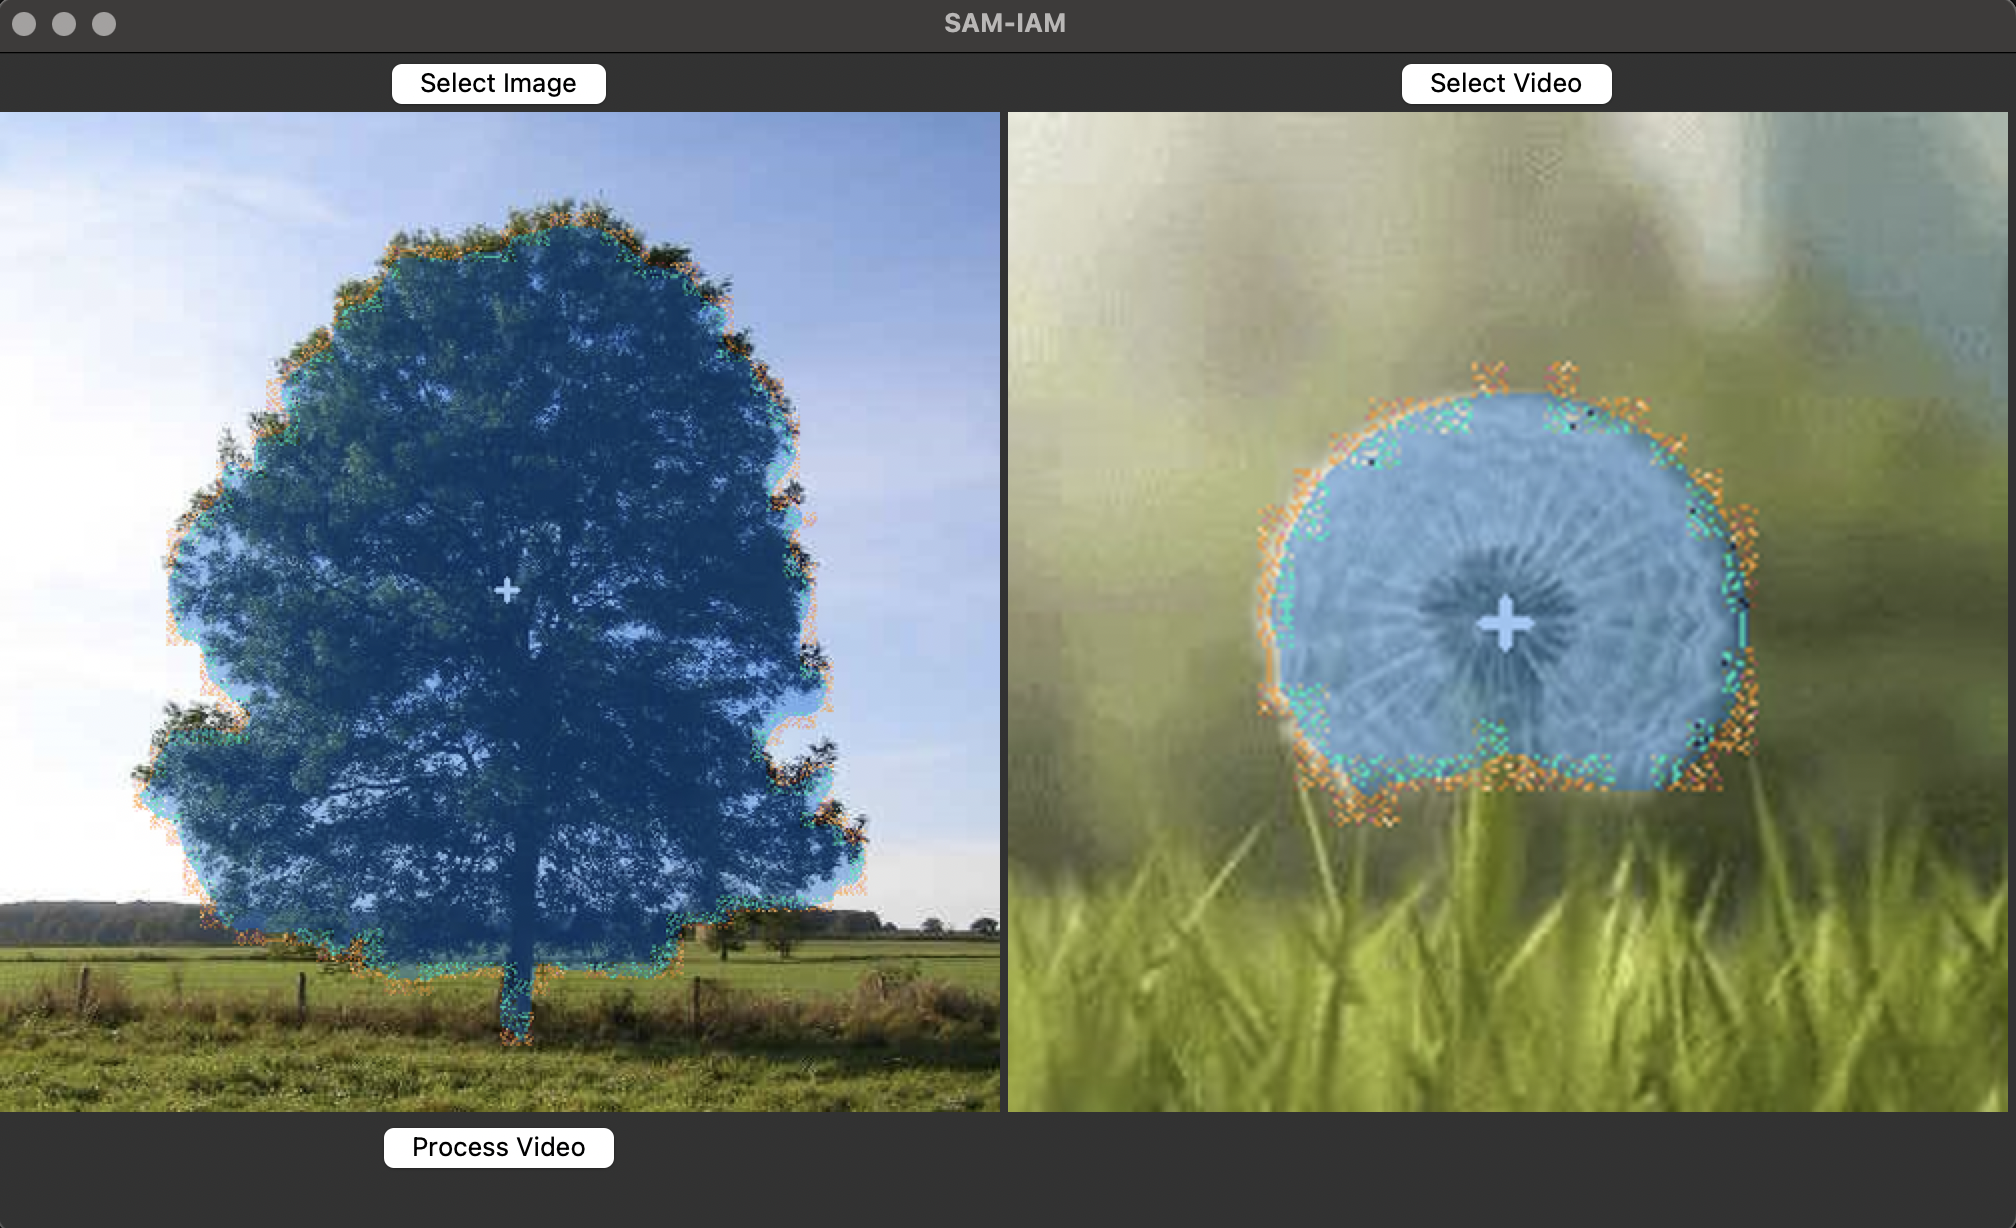
\includegraphics[width=1\linewidth]{media/ui.png}
    \caption{A screenshot of our segmentation UI.}
    \label{fig:ui}
\end{figure}

%-------------------------------------------------------------------------
\subsection{Bounding Box Motion Transfer}


Given a binary segmentation mask, it is trivial to draw a bounding box around it. We can obtain a rough estimate for the relative motion of a video by calculating the change in position and scale between each frame.
For each frame in the driving video, we obtain a translation \textit{t} and change in scale \textit{s} of its corresponding bounding box, relative to the first frame.
\begin{equation}
    \begin{gathered}
        t_{n} = (\text{bbox}_{\text{vid}_n}.x-\text{bbox}_{\text{vid}_0}.x, \text{bbox}_{\text{vid}_n}.y-\text{bbox}_{\text{vid}_0}.y) \\
        s_{n} = (\frac{\text{bbox}_{\text{vid}_n}.width}{\text{bbox}_{\text{vid}_0}.width},\frac{\text{bbox}_{\text{vid}_n}.height}{\text{bbox}_{\text{vid}_0}.height})
    \end{gathered}
    \label{eq:transformation}
\end{equation}

To preserve the direction of motion while accounting for possible differences in size, we introduce scaling factors \textit{x} and \textit{y}.
These scaling factors are equal to the height and width ratios of the bounding boxes for the input image and first frame of the driving video.
\begin{equation}
    \begin{gathered}
        x = \frac{\text{bbox}_\text{img}.width}{\text{bbox}_\text{vid}.width} \\ y = \frac{\text{bbox}_\text{img}.height}{\text{bbox}_\text{vid}.height}
    \end{gathered}
    \label{eq:scaling}
\end{equation}

We sequentially apply the adjusted set of translations and scales to the mask of the input image to obtain a target video \textit{V}, which we use as input for a conditional diffusion model\cite{2023videocomposer}.
\begin{equation}
    \begin{gathered}
        V_{n}.size = \text{bbox}_\text{img}.size*s_{n}*(x,y) \\
        V_{n}.pos = \text{bbox}_\text{img}.pos + t_{n}*(x,y) \\
        V_{n}.pos = V_{n}.pos - \frac{(V_{n}.size-\text{bbox}_{n}.size)}{2}
    \end{gathered}
\end{equation}
